\documentclass[11pt,a4paper]{article}
\usepackage[margin=25mm,headheight=15pt]{geometry}
\usepackage[T1]{fontenc}
\usepackage{newtxtext}
\usepackage{mathtools,amsthm}
\usepackage{newtxmath}
\usepackage{microtype,graphicx,booktabs,array,longtable,aliascnt}
\usepackage{xcolor,fancyhdr,enumitem,xurl}
\usepackage[colorlinks=true,linkcolor=blue!35!black,citecolor=blue!35!black,urlcolor=blue!35!black]{hyperref}
\usepackage[nameinlink,noabbrev]{cleveref}
\hypersetup{pdftitle={Direct Optimal Truncation of Inverse Harmonic Transseries},pdfauthor={Research article prepared for Vladimir Reshetnikov},pdfsubject={Reflection, positive tail densities, and eventual enveloping}}
\setlength{\parskip}{4pt}
\setlength{\parindent}{1.25em}
\setlength{\emergencystretch}{2em}
\allowdisplaybreaks[1]
\pagestyle{fancy}
\fancyhf{}
\fancyhead[L]{\small Direct inverse-harmonic truncation}
\fancyhead[R]{\small ProveIt research extension}
\fancyfoot[C]{\thepage}
\renewcommand{\headrulewidth}{0.3pt}
\newtheorem{theorem}{Theorem}[section]
\newaliascnt{lemma}{theorem}
\newtheorem{lemma}[lemma]{Lemma}
\aliascntresetthe{lemma}
\newaliascnt{proposition}{theorem}
\newtheorem{proposition}[proposition]{Proposition}
\aliascntresetthe{proposition}
\newaliascnt{corollary}{theorem}
\newtheorem{corollary}[corollary]{Corollary}
\aliascntresetthe{corollary}
\theoremstyle{definition}
\newaliascnt{definition}{theorem}
\newtheorem{definition}[definition]{Definition}
\aliascntresetthe{definition}
\newaliascnt{remark}{theorem}
\newtheorem{remark}[remark]{Remark}
\aliascntresetthe{remark}
\newtheorem{problem}{Research question}
\crefname{lemma}{lemma}{lemmas}
\Crefname{lemma}{Lemma}{Lemmas}
\crefname{proposition}{proposition}{propositions}
\Crefname{proposition}{Proposition}{Propositions}
\crefname{corollary}{corollary}{corollaries}
\Crefname{corollary}{Corollary}{Corollaries}
\crefname{definition}{definition}{definitions}
\Crefname{definition}{Definition}{Definitions}
\crefname{remark}{remark}{remarks}
\Crefname{remark}{Remark}{Remarks}

\numberwithin{equation}{section}
\newcommand{\dd}{\mathop{}\!\mathrm{d}}
\newcommand{\ii}{\mathrm{i}}
\newcommand{\ee}{\mathrm{e}}
\newcommand{\Oh}{\mathcal O}
\newcommand{\R}{\mathbb R}
\newcommand{\C}{\mathbb C}
\newcommand{\N}{\mathbb N}
\newcommand{\coef}[2]{[#1^{#2}]}
\newcommand{\cformal}{\mathscr C}
\newcommand{\Wformal}{\widetilde W}
\newcommand{\Vformal}{\widetilde V}
\newcommand{\Dformal}{\widetilde D}
\newcommand{\E}{\mathbb E}
\newcommand{\repo}{\textit{ProveIt}}
\newcommand{\ctail}{\mathcal E}
\newcommand{\rising}[2]{(#1)_{#2}}
\begin{document}
\begin{titlepage}
\vspace*{9mm}
\noindent{\large\scshape Transseries and quantitative asymptotic inversion}\par
\vspace{10mm}
\noindent{\huge\bfseries\raggedright Direct Optimal Truncation\\[2mm] of Inverse Harmonic\\[2mm] Transseries\par}
\vspace{7mm}
\noindent{\Large Reflection, positive tail densities,\\[1mm] and eventual enveloping\par}
\vspace{10mm}
\noindent Research article prepared for Vladimir Reshetnikov\par
\noindent 29 September 2026\par
\vspace{8mm}\hrule\vspace{5mm}
\begin{abstract}
Let $W(X)$ be the positive solution of $\psi(W+\tfrac12)=\log X$, and let
$S_N(X)=X+\sum_{n=1}^Nh_nX^{1-2n}$ be its direct asymptotic partial sum.
The \repo\ inverse-harmonic report explicitly leaves open a signed
first-omitted-term bound for these sums and their sharp error when
$N-\pi X$ is bounded. We resolve the latter question and establish the
former on an eventual domain uniform in both $X$ and $N$.

The key step is an exterior dispersion representation. Digamma reflection
identifies the difference between two sectorial inverse branches and produces
an eventually positive density
$\rho(t)=-2\operatorname{Re}W_R(\ii t)/\pi\sim2t\ee^{-2\pi t}$.
The inverse is a Stieltjes-type tail integral plus a convergent odd Laurent
correction. This representation yields an exact direct remainder and proves
that, for suitable $X_0,N_0$, every $X\ge X_0$ and $N\ge N_0$ satisfies
$0<(-1)^N(S_N-W)<|h_{N+1}|X^{-2N-1}$.

For $\sigma=N+1-\pi X$ bounded, the sharp error is
\[
 S_N-W=(-1)^N\sqrt X\,\ee^{-2\pi X}
 \left\{1+\frac1X\left[-\frac\pi{12}
 +\frac{2\sigma^2-3\sigma+7/12}{2\pi}\right]
 +\Oh(X^{-2})\right\}.
\]
We prove an all-orders extension, give the next explicit coefficient,
identify the half-next-term law and a square-root truncation window,
and quantify the first difference from forward-truncation inversion.
Exact rational sign certificates and 190-digit experiments accompany the proofs.
\end{abstract}
\vspace{3mm}
\noindent\textbf{Scope.} The thresholds in the uniform enveloping theorem are
existential, with an explicit sufficient criterion in analytic constants;
no numerical global threshold is asserted. The proofs are not Lean-checked.
Priority beyond the inspected repository and the cited literature is not established.
\vfill
\noindent\small Pinned repository snapshot:
\texttt{a795fcffa4b3ece22761d81fbed3c43be8b81795}.
\end{titlepage}
\begingroup\small\setlength{\parskip}{0pt}\tableofcontents\endgroup
\newpage

\section{The question, the answer, and its boundary}
\label{sec:introduction}

\subsection{Two approximations that must not be confused}
For a divergent inverse expansion, truncating and inverting need not commute
at exponentially small scales. This distinction is central here. Put
\begin{equation}
 F(w)=\psi(w+\tfrac12),\qquad F(W(X))=\log X,
 \label{eq:normalization}
\end{equation}
where $\psi$ is the digamma function and $X$ is large and positive.
The usual harmonic interpolation $H(x)=\psi(x+1)+\gamma$ is recovered through
\begin{equation}
 H^{-1}(y)=W(\ee^{y-\gamma})-\tfrac12.
 \label{eq:harmonic}
\end{equation}
The centering by one half makes the formal inverse odd:
\begin{equation}
 \Wformal(X)=X+\sum_{n\ge1}h_nX^{1-2n}.
 \label{eq:formalW}
\end{equation}
One may either take its direct partial sum $S_N$, or truncate the forward
expansion of $F$ and solve that truncated equation. We denote the latter
root by $u_N$. These are different functions of $X$ even though they have
many identical algebraic expansion terms.

The predecessor report, \emph{Exponential Accuracy and Stokes Transport for
Inverse Harmonic Transseries} \cite{prior}, proves a sharp exponential error
for $u_N$, as well as all-order large-coefficient asymptotics and inverse
Stokes-sector formulas. Its problem labelled \texttt{prob:direct}, entitled
``Direct inverse partial sums and an enveloping law'', explicitly asks for
the corresponding signed bound and sharp error for $S_N$. The report
correctly warns that positivity of a forward remainder is not a proof of
positivity after nonlinear inversion. This article supplies a separate
analytic argument for the direct sums.

\subsection{Main conclusions}
Our exact representation is
\begin{equation}
 W(X)=X+E_T(X)-X\int_T^\infty\frac{\rho(t)}{X^2+t^2}\dd t,
 \label{eq:intro-dispersion}
\end{equation}
where $T$ is sufficiently large, $E_T$ is an odd Laurent series convergent
for $|X|>T$, and $\rho(t)>0$ for $t\ge T$. Importantly, we do not discard
$E_T$. It contains the effect of the bounded part of the continuation
geometry and cannot be presumed to vanish.

\Cref{thm:dispersion,thm:remainder} give the representation and the exact
remainder. \Cref{thm:enveloping} proves a first-omitted-term bound on a
rectangle $X\ge X_0$, $N\ge N_0$. \Cref{thm:sharp} gives every algebraic
correction to the optimal-scale error. \Cref{thm:macro,thm:sqrt} describe
larger truncation windows. Finally, \cref{cor:comparison} proves
\begin{equation}
 S_N(X)-u_N(X)=(-1)^{N+1}\frac\pi6 X^{-1/2}\ee^{-2\pi X}
                   \bigl(1+\Oh(X^{-1})\bigr)
 \label{eq:intro-comparison}
\end{equation}
when $N-\pi X$ is bounded. Thus agreement of the leading exponential
constant does not make the two approximation procedures interchangeable.

\subsection{What is and is not new in the argument}
The coefficient formula for $h_n$ and its fixed-order asymptotic meaning
come from the repository's combinatorial companion \cite{companion}.
Reflection, the centered digamma expansion, Binet's formula, and Stirling's
formula are classical \cite{dlmf55,dlmf59,dlmf511}. Formal reversion and
factorial asymptotics have extensive existing theories; Fabijonas and Olver
\cite{fo} and Borinsky \cite{borinsky} are relevant background. Nemes
\cite{nemes} proves enveloping results for reverted cylinder- and Airy-zero
expansions by studying analytic inverse functions. That work is a close
methodological precedent, not a theorem about the present harmonic inverse.

The contribution developed here is the particular reflected inverse
jump, its positive tail density, the retained convergent correction, and
the resulting direct-remainder theorems for this family. Our argument does
not require a general resurgent-closure theorem. In particular, a
positive-real least-term error is not identified with a positive-real
Stokes jump: the branch comparison used below is on the imaginary axis.
The large-order coefficient result derived from the density is an
independent recovery of a result already established in \cite{prior}, not
an additional claim of priority.

The exact proposition answered is a repository research question. Neither
its phrasing there nor the targeted literature check establishes that it
was a previously named open problem throughout the wider literature.
Likewise, the article is a mathematical proof submission with reproducible
finite checks, not a declaration of formal verification or independent
peer review.

\subsection{Notation and quantifiers}
We write $A=2\pi$ throughout. The letter $N$ is the number of retained
inverse terms; the first omitted term has index $N+1$. The bounded-shift
parameter is
\begin{equation}
 \sigma=N+1-\pi X.
 \label{eq:sigma}
\end{equation}
All error bounds involving bounded $\sigma$ are uniform on any specified
compact interval of its values. An all-orders expansion means a separate
proved bound for every fixed requested order, not convergence of the
resulting formal series.

The real inverse is $W$; the right and left sectorial branches are $W_R$
and $W_L$. Tildes distinguish formal series from functions.
$E_T$ is an actual convergent Laurent correction, while
$\ctail_N$ is its tail after $N$ terms. The exact positive direct-remainder
integral is denoted by $A_N(X)$; it is not the constant $A$.

\section{The formal coefficients and the sectorial inverse}
\label{sec:inverse}

\subsection{Centered coefficients and formal reversion}
Define
\begin{equation}
 \cformal(z)=\sum_{j\ge1}c_jz^j,\qquad
 c_j=-\frac{B_{2j}(1/2)}{2j}.
 \label{eq:c}
\end{equation}
The centered digamma expansion, obtained from the standard shifted
expansion \cite{dlmf511}, is
\begin{equation}
 F(w)\sim\log w+\cformal(w^{-2})
 \quad (|w|\to\infty,\ |\arg w|\le\theta_0<\pi).
 \label{eq:centered}
\end{equation}
The first coefficients are
\begin{equation}
 c_1=\frac1{24},\quad c_2=-\frac7{960},\quad
 c_3=\frac{31}{8064},\quad c_4=-\frac{127}{30720}.
 \label{eq:cfirst}
\end{equation}
Every fixed truncation has a uniform remainder on a slightly smaller
closed sector. Cauchy's formula on disks with radius proportional to
$|w|$ then permits termwise differentiation of any such fixed truncation.
No assertion about uniformity in an unbounded truncation order is made here.

\begin{proposition}[The inherited inverse coefficient formula]
\label{prop:coefficients}
There is a unique formal odd Laurent solution of
$\log(\Wformal/X)+\cformal(\Wformal^{-2})=0$. Its coefficients are
\begin{equation}
 h_n=-\frac1{2n-1}\coef{z}{n}
       \exp\bigl((2n-1)\cformal(z)\bigr),\qquad n\ge1.
 \label{eq:h}
\end{equation}
The first five are
\begin{equation}
 h_1=-\frac1{24},\quad h_2=\frac3{640},\quad
 h_3=-\frac{1525}{580608},\quad
 h_4=\frac{615881}{199065600},\quad
 h_5=-\frac{3058641}{504627200}.
 \label{eq:hfirst}
\end{equation}
\end{proposition}
\begin{proof}
Put $v=\Wformal^{-1}$ and $t=X^{-1}$. The equation becomes
$v=t\exp(\cformal(v^2))$. Formal Lagrange inversion gives its unique odd
power-series solution. The Laurent version of the coefficient formula is
\[
 \coef{t}{2n-1}\frac1{v(t)}
 =-\frac1{2n-1}\coef{u}{2n}
       \exp\bigl((2n-1)\cformal(u^2)\bigr),
\]
which proves \eqref{eq:h}. This identity can also be verified by the
formal-residue substitution $t=v\exp(-\cformal(v^2))$.
The displayed rational values follow by finite coefficient extraction.
This is the normalization used in the companion \cite{companion}.
\end{proof}

\subsection{A local-at-infinity inverse, not global univalence}
Exponentiating the forward phase removes the logarithm:
\begin{equation}
 G(w)=\exp\psi(w+\tfrac12).
 \label{eq:G}
\end{equation}
It follows from \eqref{eq:centered} that, uniformly on every closed
sector strictly inside the cut plane,
\begin{equation}
 G(w)=w+\Oh(w^{-1}),\quad G'(w)=1+\Oh(w^{-2}),\quad
 G''(w)=\Oh(w^{-3}).
 \label{eq:Gnear}
\end{equation}
The poles of the digamma function on the negative real axis play no role
in these sectors.

\begin{lemma}[The right inverse branch]
\label{lem:sector}
Fix $\pi/2<\theta<\theta_0<\pi$. For some $R>0$ there is a holomorphic
function $W_R$ on
\[
 \mathcal S_R=\{z:|z|>R,\ |\arg z|<\theta\}
\]
such that $G(W_R(z))=z$ and $W_R(z)=z+\Oh(z^{-1})$.
It is the unique solution sufficiently close to $z$, it satisfies
\begin{equation}
 W_R(\overline z)=\overline{W_R(z)},\qquad
 W_R'(z)=\frac1{G'(W_R(z))}=1+\Oh(z^{-2}),
 \label{eq:Wderivative}
\end{equation}
and, for every fixed $m$,
\begin{equation}
 W_R(z)=z+\sum_{n=1}^m h_nz^{1-2n}+\Oh_m(|z|^{-2m-1})
 \label{eq:Wsector}
\end{equation}
uniformly on a smaller closed sector. On the positive real axis it is
the inverse in \eqref{eq:normalization}.
\end{lemma}
\begin{proof}
For large $z$ in the specified sector, a disk of radius $K/|z|$ centered
at $z$ lies in the larger sector. On its boundary,
$G(w)-z=(w-z)+\Oh(|z|^{-1})$. Choose $K$ larger than a uniform constant
in this bound. Rouch\'e's theorem then gives exactly one zero in the disk.
The derivative estimate in \eqref{eq:Gnear} makes it a simple zero.
The implicit-function theorem gives a holomorphic solution locally in
$z$, and uniqueness in the disks identifies the local solutions on overlaps.
This constructs the branch without asserting that $G$ is globally injective.

Conjugation and uniqueness give the first identity in
\eqref{eq:Wderivative}; differentiation of $G(W_R)=z$ gives the second.
Substitution of a fixed formal truncation from \cref{prop:coefficients}
into $G$ leaves an error $\Oh_m(z^{-2m-1})$. Its actual inverse derivative
is uniformly bounded, or equivalently the same small-disk argument applies
to the residual. This proves \eqref{eq:Wsector}. Derivatives follow by
Cauchy estimates in a slightly smaller sector.

Finally, $F(W_R(z))-\log z$ is an integer multiple of $2\pi\ii$,
but its asymptotic size is $\Oh(z^{-2})$; hence it is zero. For positive
large $z$ the solution is real and positive. The standard trigamma series
\cite{dlmf59} gives
\begin{equation}
 F'(w)=\sum_{k=0}^\infty(w+\tfrac12+k)^{-2}>0\qquad(w>0),
 \label{eq:monotone}
\end{equation}
so this solution agrees with the positive real inverse.
\end{proof}

Define the reflected branch by
\begin{equation}
 W_L(z)=-W_R(-z),\qquad K(w)=-G(-w).
 \label{eq:left}
\end{equation}
Then $K(W_L(z))=z$. Its sector contains the exterior left half-plane.
Both branches are defined near each sufficiently high point of the
imaginary axis. Their formal odd expansions agree there; their exact
functions need not agree. This is precisely the exponentially small
information used next.

\section{Reflection and the positive inverse-jump density}
\label{sec:density}

\subsection{The exact reflected forward map}
The digamma reflection identity \cite{dlmf55} implies
\begin{equation}
 \psi(\tfrac12-w)=\psi(\tfrac12+w)-\pi\tan(\pi w).
 \label{eq:reflectionpsi}
\end{equation}
For $\operatorname{Im}w>0$ set $q=\ee^{2\pi\ii w}$. Since
$\tan(\pi w)=\ii(1-q)/(1+q)$, exponentiation gives the exact identity
\begin{equation}
 K(w)=G(w)\exp J(w),\qquad
 J(w)=\frac{A\ii q}{1+q},\qquad A=2\pi.
 \label{eq:reflectionG}
\end{equation}
The minus sign in the definition of $K$ cancels the factor
$\exp(-\pi\ii)=-1$. Losing that sign would reverse the density below.

\begin{lemma}[Leading reflected inverse jump]
\label{lem:jump}
Let $z$ lie in a fixed-width strip about the positive imaginary axis,
and put $t=\operatorname{Im}z\to+\infty$. Then
\begin{equation}
 W_R(z)-W_L(z)
 =A\ii zW_R'(z)\exp\bigl(A\ii W_R(z)\bigr)
      +\Oh(t^2\ee^{-2At}).
 \label{eq:jump}
\end{equation}
The error is uniform in each fixed-width strip. The jump and its first
derivative are $\Oh(t\ee^{-At})$ there.
\end{lemma}
\begin{proof}
Write $w=W_R(z)$, $v=W_L(z)$, and $\Delta=w-v$. Both $w$ and $v$
are within $\Oh(t^{-1})$ of $z$, and $q(w)=\Oh(\ee^{-At})$.
By \eqref{eq:reflectionG},
\[
 K(w)-K(v)=z\{\exp J(w)-1\}.
\]
On the segment between $v$ and $w$, $K'=1+\Oh(t^{-2})$.
The integral of this derivative along the segment is bounded away from
zero, so the preceding equation first gives
$\Delta=\Oh(t\ee^{-At})$. Taylor expansion now gives
\[
 K'(w)\Delta=z\{\exp J(w)-1\}
              +\Oh(t^{-3}\Delta^2).
\]
Also $K'(w)=G'(w)+\Oh(t\ee^{-At})$ and
$\exp J(w)-1=A\ii q(w)+\Oh(q(w)^2)$.
Division by $G'(w)$, using $1/G'(w)=W_R'(z)$, proves
\eqref{eq:jump}. All estimates remain valid on a slightly wider strip.
Cauchy's derivative estimate on fixed-radius disks then bounds the
derivative of the jump by $\Oh(t\ee^{-At})$ as well.
\end{proof}

\subsection{The density and every algebraic coefficient of its tail}
At $z=\ii t$, conjugation gives
$W_L(\ii t)=-\overline{W_R(\ii t)}$. Consequently the jump is real.
Define the exact real function
\begin{equation}
 \rho(t)=-\frac{W_R(\ii t)-W_L(\ii t)}\pi
         =-\frac2\pi\operatorname{Re}W_R(\ii t).
 \label{eq:rho}
\end{equation}
This definition is used only for sufficiently large positive $t$.

For the algebraic tail coefficients define the formal series
\begin{align}
 \Vformal(t)&=-\ii\Wformal(\ii t)
     =t+\sum_{n\ge1}(-1)^nh_nt^{1-2n},\label{eq:V}\\
 \Dformal(t)&=\Vformal'(t)
                \exp\{-A(\Vformal(t)-t)\}
       =\sum_{j\ge0}d_jt^{-j}.\label{eq:D}
\end{align}
In particular,
\begin{equation}
 \Vformal(t)=t+\frac1{24t}+\frac3{640t^3}
                  +\frac{1525}{580608t^5}+\cdots.
 \label{eq:Vfirst}
\end{equation}

\begin{theorem}[Positive tail density]
\label{thm:density}
There exists $T$ such that $\rho(t)>0$ for all $t\ge T$.
For every fixed $J\ge1$,
\begin{equation}
 \rho(t)=2t\ee^{-At}
 \left(\sum_{j=0}^{J-1}\frac{d_j}{t^j}+\Oh_J(t^{-J})\right),
 \label{eq:rhoasympt}
\end{equation}
where the coefficients are exactly those of \eqref{eq:D}.
Furthermore $\rho(t),\rho'(t)=\Oh(t\ee^{-At})$.
The first coefficients are
\begin{align}
 d_0&=1,&d_1&=-\frac\pi{12},\label{eq:d01}\\
 d_2&=\frac{\pi^2}{288}-\frac1{24},&
 d_3&=-\frac{17\pi}{2880}-\frac{\pi^3}{10368},\label{eq:d23}\\
 d_4&=-\frac9{640}+\frac{11\pi^2}{17280}
                         +\frac{\pi^4}{497664}.\label{eq:d4}
\end{align}
\end{theorem}
\begin{proof}
At $z=\ii t$, the principal term in \eqref{eq:jump} is
$-AtW_R'(\ii t)\exp(A\ii W_R(\ii t))$.
Every fixed algebraic expansion of $-\ii W_R(\ii t)$ is the corresponding
truncation of $\Vformal(t)$, and the derivative expansion of
$W_R'(\ii t)$ is $\Vformal'(t)$. Dividing the jump by $-\pi$ therefore gives
\eqref{eq:rhoasympt}. To justify a requested order, take sufficiently many
terms in the uniform expansion \eqref{eq:Wsector}, then use finite Taylor
expansions of the exponential and derivative. The error term from
\eqref{eq:jump}, relative to $2t\ee^{-At}$, is
$\Oh(t\ee^{-At})$, smaller than every fixed inverse power of $t$.
No summation of the generally divergent formal series $\Vformal$ is used.

The leading coefficient is one, so the exact real density is eventually
positive. Smoothness and the derivative bound follow from \cref{lem:jump}.
Finally, expand \eqref{eq:D} using \eqref{eq:Vfirst}; this gives
\eqref{eq:d01}--\eqref{eq:d4} by finite algebra.
\end{proof}

\begin{remark}[Why algebraic asymptotics alone would not suffice]
Every coefficient of $W_R(\ii t)$ in its inverse-power expansion is purely
imaginary. Thus that expansion alone cannot decide the sign of its real
part. The exact reflection identity and the comparison of two actual
inverse branches are essential. They fix the leading exponentially small
real part, and hence the sign of $\rho$, rather than merely suggesting it
from a truncated formal expression.
\end{remark}

\section{An exterior dispersion representation}
\label{sec:dispersion}

\subsection{Keeping the bounded part of the continuation problem}
Choose $T$ large enough that both sectorial branches exist on the relevant
closed half-circles of radius $T$, and that the density is positive for
$t\ge T$. On the exterior right and left half-planes, respectively, set
\begin{equation}
 f_R(z)=W_R(z)-z,\qquad f_L(z)=W_L(z)-z.
 \label{eq:fbranches}
\end{equation}
Write $f$ for this piecewise function, using $f_R$ on the right and $f_L$
on the left. Values at the two cut points of the circle may be assigned
arbitrarily for integration. Define
\begin{equation}
 E_T(z)=-\frac1{2\pi\ii}\int_{|\zeta|=T}^{\mathrm{ccw}}
                  \frac{f(\zeta)}{\zeta-z}\dd\zeta,
       \qquad |z|>T.
 \label{eq:Econtour}
\end{equation}
This is an ordinary finite contour integral of a bounded piecewise
analytic boundary function. It defines a holomorphic function throughout
the exterior disk, even though the boundary function itself has two jumps.
Let
\begin{equation}
 M_T=\sup_{\substack{|\zeta|=T\\\operatorname{Re}\zeta\ne0}}
                        |f(\zeta)|<\infty.
 \label{eq:MT}
\end{equation}
The one-sided boundary values are bounded as well.

\begin{theorem}[Exterior dispersion with a convergent correction]
\label{thm:dispersion}
For $z$ in either exterior half-plane,
\begin{equation}
 f(z)=E_T(z)-z\int_T^\infty\frac{\rho(t)}{z^2+t^2}\dd t.
 \label{eq:dispersion}
\end{equation}
The function $E_T$ is odd, has real Laurent coefficients, and has the
convergent expansion
\begin{equation}
 E_T(z)=\sum_{n\ge1}e_nz^{1-2n},\qquad |z|>T,
 \label{eq:Elau}
\end{equation}
with
\begin{equation}
 |e_n|\le M_TT^{2n-1}.
 \label{eq:ebound}
\end{equation}
In particular, \eqref{eq:intro-dispersion} holds for every real $X>T$.
\end{theorem}
\begin{proof}
Apply Cauchy's formula separately to the right and left half-annuli
$T<|\zeta|<R$, and add the results. If $z$ is in the right half-annulus,
its Cauchy term occurs only in that half-annulus; the left one contributes
zero. The same argument works with right and left interchanged.

The inner circular contribution is exactly \eqref{eq:Econtour}. The outer
circular contribution tends to zero as $R\to\infty$: uniformly on its two
half-circles, $f(\zeta)=\Oh(R^{-1})$, while
$(\zeta-z)^{-1}=\Oh(R^{-1})$ and the total arc length is $2\pi R$.
We are left with the two integrals along the imaginary-axis boundaries.
Their convergence follows from the exponential jump bound.

For completeness, keep track of their signs. On the upper imaginary
axis the right boundary is traversed downward and the left boundary
upward. Their sum is
\[
 -\frac1{2\pi\ii}\int_{\ii T}^{\ii\infty}
          \frac{f_R(\zeta)-f_L(\zeta)}{\zeta-z}\dd\zeta
   =\frac12\int_T^\infty\frac{\rho(t)}{\ii t-z}\dd t.
\]
Conjugation gives the same real jump $-\pi\rho(t)$ at $-\ii t$.
The lower boundary contribution is consequently
\[
 \frac12\int_T^\infty\frac{\rho(t)}{-\ii t-z}\dd t.
\]
Adding the two kernels gives $-z/(z^2+t^2)$, proving
\eqref{eq:dispersion}. This contour argument avoids any assumption that
the inverse extends through the bounded disk.

The symmetries $f(-\zeta)=-f(\zeta)$ and
$f(\overline\zeta)=\overline{f(\zeta)}$ follow from the definitions of the
branches. The integral correction has the same symmetries, so $E_T$ is
odd and real-symmetric. Alternatively, they follow directly from
\eqref{eq:Econtour}. Expanding its kernel for $|z|>T$ gives
\[
 e_n=\frac1{2\pi\ii}\int_{|\zeta|=T}^{\mathrm{ccw}}
                  f(\zeta)\zeta^{2n-2}\dd\zeta.
\]
The coefficients of the even negative powers vanish by oddness.
The arc-length bound gives \eqref{eq:ebound} and proves convergence.
\end{proof}

\begin{remark}[This is not a global Stieltjes assertion]
The representation contains a positive Stieltjes-type tail, not a claim
that $X-W(X)$ is a Stieltjes transform on its full natural domain.
The finite contour correction $E_T$ may be nonzero. Positivity is proved
only for the tail density after a sufficiently large cutoff. These two
restrictions are exactly what make a local-at-infinity argument enough;
a global study of all critical points of the digamma inverse is unnecessary.
\end{remark}

The decomposition is not unique in its cutoff. If $T'>T$ is also
admissible, then
\begin{equation}
 E_{T'}(z)=E_T(z)-z\int_T^{T'}\frac{\rho(t)}{z^2+t^2}\dd t
 \qquad (|z|>T').
 \label{eq:cutoffchange}
\end{equation}
Thus changing the cutoff only moves a compact piece of the integral into
a convergent Laurent series. The full function and its asymptotic
coefficients are unchanged.

\subsection{Exact moments and the direct remainder}
All moments
\begin{equation}
 \mu_k=\int_T^\infty\rho(t)t^k\dd t\qquad(k\ge0)
 \label{eq:moments}
\end{equation}
are finite and positive. Define the convergent correction tail by
\begin{equation}
 \ctail_N(X)=E_T(X)-\sum_{n=1}^Ne_nX^{1-2n}.
 \label{eq:E-tail}
\end{equation}
For $N=0$, the empty sum is zero.

\begin{theorem}[Moment coefficients and an exact direct remainder]
\label{thm:remainder}
For every $n\ge1$,
\begin{equation}
 h_n=e_n+(-1)^n\mu_{2n-2}.
 \label{eq:hmoments}
\end{equation}
For every $X>T$ and integer $N\ge0$,
\begin{align}
 S_N(X)-W(X)&=(-1)^N A_N(X)-\ctail_N(X),\label{eq:exact-remainder}\\
 A_N(X)&=X^{-2N-1}\int_T^\infty
        \frac{\rho(t)t^{2N}}{1+(t/X)^2}\dd t>0,\label{eq:AN}\\
 |\ctail_N(X)|&\le
       \frac{M_T(T/X)^{2N+1}}{1-(T/X)^2}.\label{eq:E-tail-bound}
\end{align}
\end{theorem}
\begin{proof}
Use the finite geometric identity
\[
 \frac1{1+u}=\sum_{k=0}^{N-1}(-u)^k+\frac{(-u)^N}{1+u}
 \qquad(u\ge0)
\]
in the integral of \eqref{eq:dispersion}. Every term is integrable.
For fixed $N$, the remaining integral is bounded by
$X^{-2N-1}\mu_{2N}$, so this is also a genuine fixed-order asymptotic
expansion. Its coefficients must agree with the unique coefficients in
\eqref{eq:Wsector}, giving \eqref{eq:hmoments}. Subtraction gives
\eqref{eq:exact-remainder} with the stated sign. Summing the geometric
majorant \eqref{eq:ebound} proves \eqref{eq:E-tail-bound}.
\end{proof}

The exact remainder is the central analytic input that fixed-order
reversion did not supply. Unlike a big-O statement with an unspecified
constant depending on $N$, it remains valid with its displayed bound for
every $N$. In particular, it can be analyzed when $N$ grows proportionally
to $X$, or when $N$ and $X$ vary independently.

\section{A uniform eventual enveloping theorem}
\label{sec:enveloping}

The convergent correction can destroy a global sign argument at small
orders. Nevertheless, the moments of a positive unbounded tail eventually
outgrow every geometric coefficient bound. The following proof makes that
comparison uniform in the evaluation point.

\begin{theorem}[Eventual enveloping on a two-parameter rectangle]
\label{thm:enveloping}
Let $T$ be an admissible cutoff in \cref{thm:dispersion}. For every
$X_0>T$ there exists an integer $N_0$ such that, simultaneously for every
$X\ge X_0$ and $N\ge N_0$,
\begin{equation}
 0<(-1)^N\bigl(S_N(X)-W(X)\bigr)
        <|h_{N+1}|X^{-2N-1}.
 \label{eq:envelope}
\end{equation}
In this range, $h_{N+1}$ has sign $(-1)^{N+1}$, and $W(X)$ lies strictly
between the consecutive sums $S_N(X)$ and $S_{N+1}(X)$.
\end{theorem}
\begin{proof}
Fix any $L>T$ and let
$m=\int_L^{L+1}\rho(t)\dd t>0$. For every $X\ge X_0$,
\begin{equation}
 A_N(X)\ge X^{-2N-1}
       \frac{mL^{2N}}{1+((L+1)/X_0)^2}.
 \label{eq:Alower}
\end{equation}
The correction bound gives, on the same range,
\begin{equation}
 |\ctail_N(X)|\le X^{-2N-1}
       \frac{M_TT^{2N+1}}{1-(T/X_0)^2}.
 \label{eq:Eupperuniform}
\end{equation}
Since $L>T$, the ratio of the right-hand side of
\eqref{eq:Eupperuniform} to that of \eqref{eq:Alower} tends to zero
geometrically as $N\to\infty$, independently of $X$. Choose $N_0$ so
that it is strictly less than one for all $N\ge N_0$. Then
\eqref{eq:exact-remainder} proves
$(-1)^N(S_N-W)>0$ throughout the rectangle.

Apply the same assertion at $N+1$. The errors of consecutive sums have
opposite signs, so $W$ lies strictly between them. Since
$S_{N+1}-S_N=h_{N+1}X^{-2N-1}$, their distance is the magnitude of this
single term. Each error is strictly smaller than that distance.
This proves both the upper bound and the stated coefficient sign.
\end{proof}

\begin{corollary}[A sufficient threshold criterion]
\label{cor:criterion}
With $X_0,L,m,M_T$ as in the proof, it suffices to choose $N_0$ so that
\begin{equation}
 \left(\frac LT\right)^{2N_0}
 >\frac{M_TT\{1+((L+1)/X_0)^2\}}
         {m\{1-(T/X_0)^2\}}.
 \label{eq:threshold}
\end{equation}
The same inequality then holds for all $N\ge N_0$.
\end{corollary}

The criterion is explicit in analytic constants, but those constants
have not been rigorously evaluated here. The theorem is therefore not a
numerical statement such as ``all $X\ge1$ and all $N\ge1$''. The six
exact-rational examples in \cref{sec:verification} establish selected
small cases independently and do not identify $X_0$ or $N_0$.

\subsection{A reusable positive-tail principle}
The proof of \cref{thm:enveloping} used only the exact form
\eqref{eq:exact-remainder}, a geometric bound for the analytic correction,
and positive mass on an interval lying beyond its geometric radius.
It did not use the specific exponential decay constant $2\pi$.
Consequently the same eventual enveloping conclusion holds for any
function with an analogous representation and an everywhere positive tail
of unbounded support having all moments finite. This principle explains
why a bounded collection of continuation complications can be separated
from a late-order sign law. It does not show that an arbitrary nonlinear
inverse has such a positive representation; establishing that input is
the main function-specific task.

\section{Sharp optimal-scale direct truncation}
\label{sec:sharp}

\subsection{Statement including two explicit correction coefficients}
\begin{theorem}[Sharp direct remainder to all algebraic orders]
\label{thm:sharp}
Let $X\to+\infty$ and $N=N(X)$ be an integer with
$\sigma=N+1-\pi X$ bounded. For each fixed $J\ge1$ there are polynomials
$B_j^-(\sigma)$, $0\le j<J$, of degree at most $2j$, such that
\begin{equation}
 S_N(X)-W(X)=(-1)^N\sqrt X\,\ee^{-2\pi X}
  \left(\sum_{j=0}^{J-1}\frac{B_j^-(\sigma)}{X^j}
                  +\Oh_J(X^{-J})\right).
 \label{eq:sharpall}
\end{equation}
The error is uniform for $\sigma$ in any prescribed compact interval.
The first coefficients are
\begin{align}
 B_0^-(\sigma)&=1,\label{eq:B0}\\
 B_1^-(\sigma)&=-\frac\pi{12}
       +\frac{2\sigma^2-3\sigma+7/12}{2\pi},\label{eq:B1}\\
 B_2^-(\sigma)&=\frac{\pi^2}{288}-\frac{43}{288}
              -\frac{\sigma^2}{12}+\frac{5\sigma}{24}
 \notag\\
 &\quad+\frac1{\pi^2}\left(
 \frac{\sigma^4}{2}-\frac{11\sigma^3}{6}
 +\frac{5\sigma^2}{3}+\frac{\sigma}{48}-\frac{203}{1152}\right).
 \label{eq:B2}
\end{align}
Every further coefficient is determined by a finite algorithm using
\eqref{eq:D}, gamma moments, and the shifted Stirling expansion.
\end{theorem}

\subsection{The gamma-expectation reduction}
Set
\begin{equation}
 b=AX=2\pi X,\qquad s=2N+2=b+2\sigma,
 \qquad f(v)=\frac1{1+v^2}.
 \label{eq:gamma-parameters}
\end{equation}
For $t\ge T$ define the exact positive amplitude
\begin{equation}
 D(t)=\frac{\rho(t)}{2t\ee^{-At}}.
 \label{eq:exactD}
\end{equation}
This function has the asymptotic expansion \eqref{eq:D}, but the latter
is not used as an infinite convergent series. If $U$ has the gamma density
$u^{s-1}\ee^{-u}/\Gamma(s)$, direct substitution $u=At$ in
\eqref{eq:AN} gives the exact identity
\begin{equation}
 A_N(X)=2X\frac{\Gamma(s)}{b^s}
 \E\left[f(U/b)D(U/A)\,\mathbf1_{\{U\ge AT\}}\right].
 \label{eq:gammaexact}
\end{equation}
At the optimal scale, the gamma variable is concentrated near $U=b$,
so the relevant part of the density is at $t\approx X$ rather than near
the fixed cutoff.

\begin{lemma}[Uniform finite-order expansion of the expectation]
\label{lem:expectation}
For bounded $d=s-b$ and fixed $J$, the expectation in
\eqref{eq:gammaexact} has an expansion through $b^{-J+1}$ with remainder
$\Oh_J(b^{-J})$. Its coefficients are polynomials in $d$ and finite
linear combinations of $A^jd_j$. They can be calculated by Taylor
expansion at $v=1$ and the exact identities
\begin{equation}
 \E(U/b-1)^k
   =b^{-k}\sum_{\ell=0}^k\binom{k}{\ell}(-b)^{k-\ell}
                        \rising{s}{\ell}.
 \label{eq:gammamoments}
\end{equation}
The coefficient of $b^{-r}$ has degree at most $2r$ in $d$.
\end{lemma}
\begin{proof}
The amplitude $D$ is bounded on $[T,\infty)$ and, for each fixed $J$,
\[
 D(t)=\sum_{j=0}^{J-1}d_jt^{-j}+\Oh_J(t^{-J}).
\]
On $U\ge b/2$, inserting this expansion leaves a remainder
$\Oh_J(b^{-J})$ in the expectation. The part $AT\le U<b/2$ is
exponentially small in $b$, uniformly for bounded $d$, by a gamma Chernoff
bound. The same is true after multiplication by any fixed inverse power
$(U/b)^{-j}$: for example, use Cauchy--Schwarz together with
\[
 \E(U/b)^{-2j}=b^{2j}\frac{\Gamma(s-2j)}{\Gamma(s)}=\Oh_j(1)
\]
and a gamma lower-tail bound, once $s>2j$. The omitted interval
$0<U<AT$ is smaller still and affects no algebraic coefficient.
These estimates justify replacing the cutoff expectation, to any fixed
algebraic order, by
\[
 \sum_{j=0}^{J-1}d_j A^j b^{-j}
                  \E\{f(U/b)(U/b)^{-j}\}.
\]

For each summand, Taylor-expand $g_j(v)=f(v)v^{-j}$ at one on
$1/2\le v\le3/2$. On this compact interval all required derivatives are
bounded. Gamma upper and lower tails outside it are exponentially small;
the preceding negative-moment estimate also controls the lower tail for
$j>0$. Taylor's theorem through degree $2J-1$, and the even moment
$\E(U/b-1)^{2J}=\Oh_J(b^{-J})$, give a remainder of the required order.
Taking a few more terms when multiplied by a known power of $b^{-1}$ is
harmless. Identity \eqref{eq:gammamoments} follows by the binomial theorem
and $\E U^\ell=\rising{s}{\ell}$.

For the degree bound, write $U/b-1=(U-s)/b+d/b$.
A centered gamma moment of order $k$ is a polynomial in $s$ of degree
at most $\lfloor k/2\rfloor$ for $k\ge2$, with the first centered moment
zero. This follows directly by expanding the centered moment generating
function
$\exp\{s\sum_{r\ge2}t^r/r\}$.
Consequently a coefficient at $b^{-r}$ in the shifted normalized moments
can involve at most $2r$ powers of $d$. The finite Taylor operations and
the additional factors $b^{-j}$ preserve the asserted bound.
\end{proof}

\subsection{The first correction and its sign}
For $f(v)=(1+v^2)^{-1}$,
\[
 f(1)=\tfrac12,\quad f'(1)=-\tfrac12,\quad
 f''(1)=\tfrac12,\quad f'''(1)=0.
\]
With $d=2\sigma$, the gamma moments give
\begin{equation}
 \E f(U/b)=\frac12+\frac{1/4-\sigma}{b}+\Oh(b^{-2}).
 \label{eq:Ef}
\end{equation}
The density amplitude contributes
$d_1 A b^{-1}\E\{f(U/b)(U/b)^{-1}\}
=d_1A/(2b)+\Oh(b^{-2})$.
Thus the expectation in \eqref{eq:gammaexact} equals
\begin{equation}
 \frac12+\frac{1/4-\sigma+Ad_1/2}{b}+\Oh(b^{-2}).
 \label{eq:EfD}
\end{equation}
The shifted Stirling expansion \cite{dlmf511}, uniformly for bounded
$d$, gives
\begin{equation}
 \frac{\Gamma(b+d)}{b^{b+d}}
 =\sqrt{2\pi}\,b^{-1/2}\ee^{-b}
 \left(1+\frac{d^2/2-d/2+1/12}{b}+\Oh(b^{-2})\right).
 \label{eq:stirlingfirst}
\end{equation}
Since $2X\sqrt{2\pi}\,b^{-1/2}=2\sqrt X$, multiplying
\eqref{eq:EfD} and \eqref{eq:stirlingfirst} yields
\[
 A_N(X)=\sqrt X\ee^{-AX}
 \left(1+\frac{2\sigma^2-3\sigma+7/12}{AX}
                    +\frac{d_1}{X}+\Oh(X^{-2})\right).
\]
The value $d_1=-\pi/12$ explains the minus sign in \eqref{eq:B1}.
There is no substitution of a forward-truncation error in this calculation.

\subsection{Proof at all orders and the second coefficient}
\begin{proof}[Proof of \cref{thm:sharp}]
For bounded $\sigma$, the convergent correction is negligible to every
algebraic order relative to the first exponential scale. Indeed,
\eqref{eq:E-tail-bound} and $2N+1=AX+\Oh(1)$ imply
\begin{equation}
 |\ctail_N(X)|
 \le\exp\{-AX\log X+\Oh(X)\}
 =o\bigl(\sqrt X\ee^{-AX}X^{-J}\bigr)
 \label{eq:Esuper}
\end{equation}
for every fixed $J$. It therefore suffices to expand \eqref{eq:gammaexact}.
Use \cref{lem:expectation} and the finite shifted logarithmic Stirling
expansion
\begin{equation}
 \log\frac{\Gamma(b+d)}{\sqrt{2\pi}\ee^{-b}b^{b+d-1/2}}
 \sim\sum_{r\ge1}\frac{(-1)^{r+1}B_{r+1}(d)}{r(r+1)b^r}.
 \label{eq:stirlingall}
\end{equation}
Every fixed truncation is uniform for $d$ in a compact interval
\cite{dlmf511}. Expanding its exponential and multiplying the two finite
expansions proves \eqref{eq:sharpall}. Its coefficient at $b^{-r}$ has
degree at most $2r$ in $d$: a Stirling-logarithm coefficient has degree
$r+1\le2r$, and the expectation has the same bound by the lemma.
Products preserve the bound. Replacing $b$ by $AX$ and $d$ by $2\sigma$
proves the stated polynomial degree bound and the finite algorithm.

Here are enough intermediate quantities to audit the second coefficient.
Taylor expansion and the exact moments give
\begin{align*}
 \E f(U/b)
 &=\frac12+\frac{1/4-\sigma}{b}
       +\frac{\sigma^2+\sigma/2-3/8}{b^2}+\Oh(b^{-3}),\\
 \E\{f(U/b)(U/b)^{-1}\}
 &=\frac12+\frac{5/4-2\sigma}{b}+\Oh(b^{-2}),\\
 \E\{f(U/b)(U/b)^{-2}\}&=\frac12+\Oh(b^{-1}).
\end{align*}
Put $L_1=B_2(2\sigma)/2$ and $L_2=-B_3(2\sigma)/6$,
where the $B_k$ on this line are Bernoulli polynomials, not the error
coefficients $B_k^-$. The Stirling multiplier through $b^{-2}$ is
$1+L_1/b+(L_2+L_1^2/2)/b^2$.
The expectation multiplier through $b^{-2}$ has coefficients
\begin{align*}
 Q_1&=\tfrac14-\sigma+Ad_1/2,\\
 Q_2&=\sigma^2+\sigma/2-\tfrac38
                  +Ad_1(\tfrac54-2\sigma)+A^2d_2/2.
\end{align*}
Therefore
\[
 B_2^-(\sigma)=\frac{2Q_2+2L_1Q_1+L_2+L_1^2/2}{A^2}.
\]
Inserting \eqref{eq:d01}--\eqref{eq:d23} and simplifying proves
\eqref{eq:B2}. These finite simplifications are also checked by the
included symbolic program.
\end{proof}

\begin{remark}[Optimal scale versus an exact minimizing integer]
The theorem covers every integer choice with $N-\pi X$ bounded. The
continuous minimum of $B_1^-(\sigma)$ occurs at $\sigma=3/4$, suggesting
$N$ close to $\pi X-1/4$. This is an asymptotic guide. The article does
not claim that this rounded prescription is the exact best integer for
every $X$, especially near a tie between neighboring integers.
\end{remark}

\section{Large coefficients and wider truncation windows}
\label{sec:windows}

\subsection{An independent recovery of the late coefficients}
The same density determines both the coefficients and the direct error.
This provides a useful consistency test against the independent
factorial-convolution proof in the predecessor report.

\begin{corollary}[Moment form of the complete late-coefficient expansion]
\label{cor:late}
For each fixed $J\ge1$,
\begin{equation}
 h_n=\frac{2(-1)^n\Gamma(2n)}{A^{2n}}
 \left\{\sum_{j=0}^{J-1}
 \frac{d_jA^j}{(2n-1)(2n-2)\cdots(2n-j)}+\Oh_J(n^{-J})\right\},
 \label{eq:late}
\end{equation}
where the denominator of the $j=0$ term is one. In particular,
\begin{equation}
 h_n\sim\frac{2(-1)^n\Gamma(2n)}{(2\pi)^{2n}}.
 \label{eq:lateleading}
\end{equation}
\end{corollary}
\begin{proof}
Insert \eqref{eq:rhoasympt} into the moment in \eqref{eq:hmoments}.
For $n$ sufficiently large, each term can be integrated over $(0,\infty)$
instead of $(T,\infty)$ with an error at most geometric in $n$.
The resulting integrals are
$\Gamma(2n-j)/A^{2n-j}$. The amplitude remainder is bounded by a constant
times $\Gamma(2n-J)/A^{2n-J}$. The coefficient $e_n$ and the missing
compact integrals are negligible relative to this factorial scale.
Dividing by $\Gamma(2n)/A^{2n}$ proves the assertion.
\end{proof}

Expanding the first correction gives
$h_n/[2(-1)^n\Gamma(2n)/A^{2n}]=1-\pi^2/(12n)+\Oh(n^{-2})$.
This agrees with the large-order normalization in \cite{prior}.
The point here is the analytic connection to \eqref{eq:exact-remainder},
not the rediscovery of the leading factorial coefficient.

\subsection{The first-omitted-term fraction on a macroscopic window}
\begin{theorem}[A uniform truncation-ratio profile]
\label{thm:macro}
Let
\begin{equation}
 r=\frac{N+1}{\pi X}.
 \label{eq:r}
\end{equation}
As $X\to\infty$, uniformly when $r$ stays in any compact subinterval of
$(0,\infty)$,
\begin{equation}
 \frac{(-1)^N\{S_N(X)-W(X)\}}
      {|h_{N+1}|X^{-2N-1}}
       =\frac1{1+r^2}+\Oh(X^{-1}).
 \label{eq:macro}
\end{equation}
\end{theorem}
\begin{proof}
In this range $N$ is comparable to $X$. Both the coefficient correction
$e_{N+1}$ and the remainder $\ctail_N$ are negligible compared with the
positive moment scales, uniformly in $r$, by \eqref{eq:ebound} and
Stirling's formula. Thus the ratio differs negligibly from
\begin{equation}
 \frac{\int_T^\infty\rho(t)t^{2N}f(t/X)\dd t}
      {\int_T^\infty\rho(t)t^{2N}\dd t}.
 \label{eq:moment-ratio}
\end{equation}
Under $u=At$, the leading weight is gamma with shape
$s=2N+2=br$. Its normalized mean is $\E(U/b)=r$, and
$\operatorname{Var}(U/b)=r/b=\Oh(X^{-1})$. The amplitude is
$D(U/A)=1+\Oh(X^{-1})$ on a concentration interval about $r$, uniformly
when $r$ stays in a fixed compact subset of $(0,\infty)$. Outside such
an interval the gamma tails are exponentially small; fixed negative
moments control the small-$U$ part as in \cref{lem:expectation}.
Taylor's theorem for $f$, whose second derivative is bounded on the
positive axis, gives $\E f(U/b)=f(r)+\Oh(X^{-1})$.
The amplitude affects numerator and denominator by $\Oh(X^{-1})$,
so \eqref{eq:moment-ratio} equals $f(r)+\Oh(X^{-1})$.
\end{proof}

\begin{corollary}[Half the first omitted term at optimal scale]
\label{cor:half}
If $N-\pi X$ is bounded, then
\begin{equation}
 \frac{(-1)^N(S_N-W)}{|h_{N+1}|X^{-2N-1}}
                  =\frac12+\Oh(X^{-1}).
 \label{eq:half}
\end{equation}
In the same regime,
\begin{equation}
 |h_{N+1}|X^{-2N-1}
             =2\sqrt X\,\ee^{-2\pi X}\bigl(1+\Oh(X^{-1})\bigr).
 \label{eq:leastterm}
\end{equation}
\end{corollary}
The coefficient two in the least-term size and the coefficient one in the
actual error thus have a precise explanation: the remainder kernel is
$(1+(t/X)^2)^{-1}$, and its mass is concentrated at $t/X\approx1$.
It is not necessary to infer this factor from a heuristic rule about
alternating divergent series.

\subsection{A square-root window around optimal truncation}
\begin{theorem}[The square-root truncation profile]
\label{thm:sqrt}
Put
\begin{equation}
 \tau=\frac{N+1-\pi X}{\sqrt X}.
 \label{eq:tau}
\end{equation}
For every fixed $K>0$, uniformly for $|\tau|\le K$,
\begin{equation}
 \frac{(-1)^N\{S_N(X)-W(X)\}}
      {\sqrt X\,\ee^{-2\pi X}}
     =\exp(\tau^2/\pi)\bigl(1+\Oh_K(X^{-1/2})\bigr).
 \label{eq:sqrtwindow}
\end{equation}
\end{theorem}
\begin{proof}
Now $s=b+d$ with $d=2\tau\sqrt X=\Oh_K(\sqrt b)$.
Stirling's formula expanded with this growing shift gives
\begin{equation}
 \frac{\Gamma(b+d)}{b^{b+d}}
 =\sqrt{2\pi}\,b^{-1/2}\ee^{-b}
   \exp\left(\frac{d^2}{2b}\right)
              \bigl(1+\Oh_K(b^{-1/2})\bigr).
 \label{eq:moderate-stirling}
\end{equation}
Indeed, expand $(b+d-1/2)\log(1+d/b)-d$; the leading term is
$d^2/(2b)$, while the terms $-d/(2b)$ and $d^3/b^2$ are
$\Oh_K(b^{-1/2})$. The usual Stirling remainder is smaller.

The gamma variable $U/b$ has mean $1+\Oh_K(b^{-1/2})$ and variance
$\Oh_K(b^{-1})$. Hence the expectation in \eqref{eq:gammaexact} is
$1/2+\Oh_K(b^{-1/2})$; the factor $D$ changes it only by
$\Oh_K(b^{-1})$. The fixed cutoff and convergent correction are
negligible as before. Finally, $d^2/(2b)=\tau^2/\pi$, proving
\eqref{eq:sqrtwindow}.
\end{proof}

\begin{figure}[tbp]
\centering
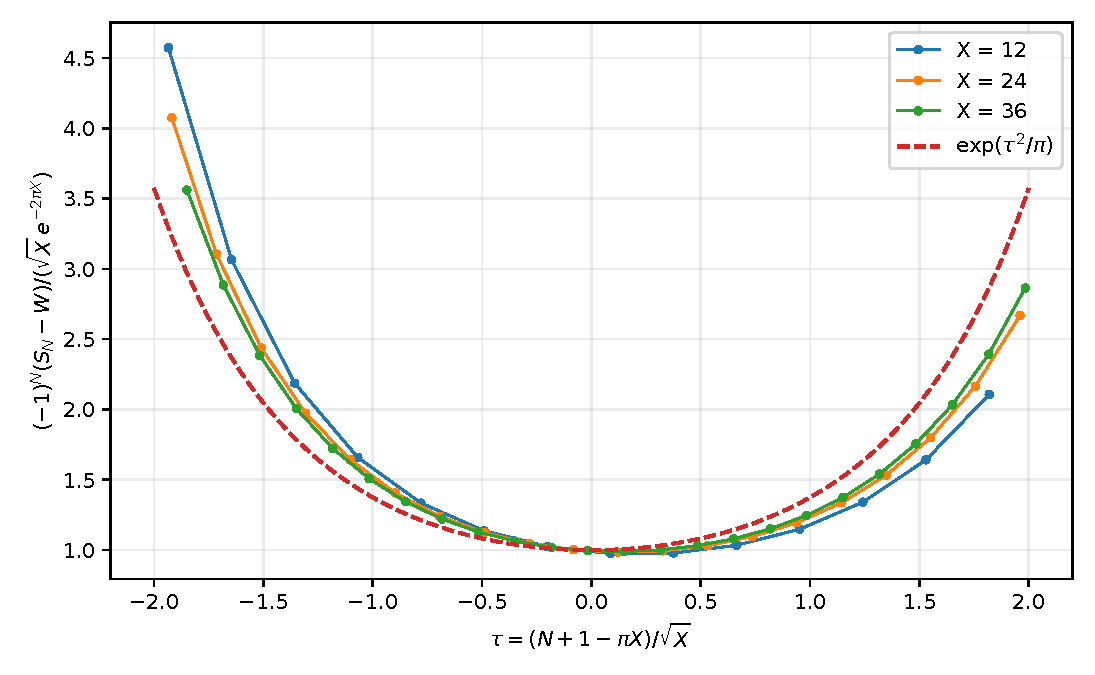
\includegraphics[width=0.94\textwidth]{figures/truncation_window.pdf}
\caption{Direct inverse errors across a square-root truncation window.
The solid curves join values calculated at integer $N$ with 190-digit
arithmetic. The dashed curve is the limiting profile in
\cref{thm:sqrt}. Visible left--right asymmetry at finite $X$ is compatible
with the stated $\Oh(X^{-1/2})$ relative correction. This is a numerical
illustration, not a substitute for the uniform proof.}
\label{fig:window}
\end{figure}

\section{Comparison with inversion of a forward truncation}
\label{sec:comparison}

\subsection{The forward integral and its signed remainder}
To make the comparison self-contained, we recall the exact forward
integral and derive the correction needed here. Binet's digamma formula
and duplication \cite{dlmf55,dlmf59} give, for $w>0$,
\begin{equation}
 C(w):=F(w)-\log w
   =2\int_0^\infty\frac{t}{w^2+t^2}\frac{\dd t}{\ee^{2\pi t}+1}.
 \label{eq:fermi}
\end{equation}
One direct derivation starts with the Bose-kernel form
\[
 \psi(w)=\log w-\frac1{2w}
      -2\int_0^\infty\frac{t}{w^2+t^2}\frac{\dd t}{\ee^{2\pi t}-1}
\]
and substitutes it into
$\psi(w+1/2)=2\psi(2w)-\psi(w)-2\log2$.
After rescaling the integral with $2w$, the kernel identity
$(\ee^u-1)^{-1}-2(\ee^{2u}-1)^{-1}=(\ee^u+1)^{-1}$ yields
\eqref{eq:fermi}.

Write
\begin{equation}
 P_N(w)=\log w+\sum_{j=1}^Nc_jw^{-2j},\qquad
 R_N(w)=F(w)-P_N(w).
 \label{eq:forward-truncation}
\end{equation}
Finite geometric expansion of \eqref{eq:fermi} gives
\begin{align}
 R_N(w)&=2(-1)^Nw^{-2N-2}\int_0^\infty
  \frac{t^{2N+1}}{1+(t/w)^2}\frac{\dd t}{\ee^{At}+1},\label{eq:forwardexact}\\
 0&<(-1)^N R_N(w)<|c_{N+1}|w^{-2N-2}.\label{eq:forwardbound}
\end{align}
The moment formula identifies the coefficients with \eqref{eq:c}.
The derivative of this exact remainder is bounded in magnitude by
$(2N+2)|R_N(w)|/w$: use the equivalent form with prefactor $w^{-2N}$
and denominator $w^2+t^2$, then differentiate under the positive integral.
A larger bound with the first omitted term in place of $|R_N|$ is
therefore valid as well.

\begin{proposition}[Forward-truncation inverse at the same scale]
\label{prop:forwardsharp}
For $N-\pi X$ bounded and $X$ sufficiently large, the equation
$P_N(u_N)=\log X$ has a unique solution near $W(X)$, and
\begin{equation}
 u_N-W=(-1)^N\sqrt X\,\ee^{-AX}
 \left(1+\frac{B_1^+(\sigma)}X+\Oh(X^{-2})\right),
 \label{eq:forwardsharp}
\end{equation}
where
\begin{equation}
 B_1^+(\sigma)=\frac\pi{12}
       +\frac{2\sigma^2-3\sigma+7/12}{2\pi}.
 \label{eq:Bplus}
\end{equation}
This is the first-correction theorem of the predecessor report
\cite{prior} in the present notation.
\end{proposition}
\begin{proof}
On an interval $w=X+\Oh(X^{-1})$ containing $W(X)$, the first omitted
forward term has size $\Oh(X^{-1/2}\ee^{-AX})$. This follows from its
explicit Bernoulli moment formula and Stirling's formula. The derivative
bound above shows that $P_N'=F'-R_N'$ is positive and asymptotic to
$X^{-1}$ there. Its residual at $W$ is $-R_N(W)$. The intermediate value
theorem therefore produces a unique local root at distance
$\Oh(\sqrt X\ee^{-AX})$. Taylor's theorem gives
\begin{equation}
 u_N-W=\frac{R_N(W)}{F'(W)}+\Oh(X\ee^{-2AX}).
 \label{eq:transportforward}
\end{equation}
For example, $F''=\Oh(X^{-2})$ and
$R_N'=\Oh(X^{-1/2}\ee^{-AX})$ give the displayed error after division
by $F'(W)\asymp X^{-1}$.

In \eqref{eq:forwardexact}, replacing $(\ee^{At}+1)^{-1}$ by
$\ee^{-At}$ changes the normalized moment by at most $2^{-2N-2}$.
The same gamma calculation as \eqref{eq:Ef}--\eqref{eq:stirlingfirst},
now with $b_w=Aw$ and $\eta=N+1-\pi w$, gives
\[
 R_N(w)=(-1)^Nw^{-1/2}\ee^{-Aw}
 \left(1+\frac{2\eta^2-3\eta+7/12}{Aw}+\Oh(w^{-2})\right).
\]
There is no density coefficient $d_1$ in this forward formula.
Finally,
\[
 W=X-\frac1{24X}+\Oh(X^{-3}),\qquad
 \frac1{F'(W)}=W\{1+\Oh(W^{-2})\}.
\]
The substitution into \eqref{eq:transportforward} introduces
$\ee^{-A(W-X)}=1+\pi/(12X)+\Oh(X^{-2})$.
This yields \eqref{eq:forwardsharp}--\eqref{eq:Bplus}.
\end{proof}

\begin{corollary}[The first discrepancy between the two procedures]
\label{cor:comparison}
Uniformly for bounded $\sigma=N+1-\pi X$,
\begin{equation}
 S_N-u_N=(-1)^{N+1}\frac\pi6 X^{-1/2}\ee^{-2\pi X}
                  \bigl(1+\Oh(X^{-1})\bigr).
 \label{eq:comparison}
\end{equation}
\end{corollary}
\begin{proof}
Subtract \eqref{eq:forwardsharp} from \eqref{eq:sharpall} through the
first correction. The leading constants cancel, while
$B_1^--B_1^+=-\pi/6$. The uniform errors are one inverse power smaller
than the nonzero difference.
\end{proof}

The direct correction and the forward correction arise from different
analytic mechanisms. The direct one contains the tail amplitude of the
reflected inverse jump. The forward one contains the exponential effect
of evaluating the forward remainder at $W(X)=X-1/(24X)+\cdots$.
The opposite signs are not an arbitrary normalization choice.

\section{Finite verification and exact-rational certificates}
\label{sec:verification}

\subsection{What was actually computed}
The accompanying program \path{verification/verify.py} performs finite
exact arithmetic checks and separate high-precision analytic diagnostics.
It generates 200 inverse coefficients numerically from the finite
exponential recurrence, computes the first 20 independently as exact
rationals, and checks the formal inverse residual through degree eight.
It then evaluates direct errors, density tails, macroscopic ratios, and
the square-root window at a total of 76 recorded parameter choices.
The main run uses 190 decimal digits. All programmed assertions passed.

For a fixed $n$, the coefficient calculation uses $E_0=1$ and
\begin{equation}
 E_k=\frac{2n-1}{k}\sum_{j=1}^k j c_j E_{k-j},\qquad
 h_n=-\frac{E_n}{2n-1}.
 \label{eq:recurrence}
\end{equation}
This is coefficient comparison in the derivative of
$\exp((2n-1)\cformal(z))$ and avoids symbolic expansion of a large
exponential. The exact residual check independently substitutes
$1+\sum_{n=1}^8h_nz^n$ into the normalized logarithmic inverse equation.

\begin{table}[tbp]
\centering\small
\begin{tabular}{rrrrr}
\toprule
$X$ & $N$ & Normalized error & Through $B_2$ & Direct/forward ratio\\
\midrule
4 & 12 & 0.9180683138 & 0.9185311808 & 1.04815277\\
8 & 25 & 0.9573226104 & 0.9573811152 & 1.02006614\\
12 & 37 & 0.9758754944 & 0.9758879980 & 1.01823786\\
20 & 62 & 0.9877449175 & 0.9877479997 & 1.01309911\\
30 & 94 & 0.9884110336 & 0.9884119587 & 1.00511017\\
40 & 125 & 0.9926247019 & 0.9926249934 & 1.00518857\\
\bottomrule
\end{tabular}

\caption{Numerical optimal-scale checks at $N=\lfloor\pi X\rfloor$.
The normalized error is $(-1)^N(S_N-W)/(\sqrt X\ee^{-2\pi X})$.
The next column is $1+B_1^-(\sigma)/X+B_2^-(\sigma)/X^2$.
The last column is
$(-1)^{N+1}(S_N-u_N)/(\pi X^{-1/2}\ee^{-2\pi X}/6)$ and tends to one.
Displayed decimals are rounded diagnostics, not interval endpoints.}
\label{tab:numeric}
\end{table}

At $X=40$, the normalized direct error is approximately
$0.99262470191319$, while the expansion through $B_2^-$ gives
$0.99262499343886$. The difference multiplied by $X^3$ is approximately
$-0.01865764$, consistent with the next bounded coefficient. Because
$\sigma$ changes with $X$, this last quantity is not expected to converge
to one constant along the displayed table.

The imaginary-axis density is particularly sensitive to precision:
$W_R(\ii t)$ has an imaginary part of size $t$ but a real part of size
$t\ee^{-2\pi t}$. At $t=40$, the computed density is approximately
$5.6250672202997191\cdot10^{-108}$. The program uses the defining
complex digamma equation at high precision and independently checks
\eqref{eq:reflectionG}. These checks support the sign and normalization;
the proof of positivity for all sufficiently large $t$ is
\cref{thm:density}, not the finite data.

\subsection{Exact sign checks without floating-point digamma values}
A rational candidate $v>0$ can be tested using only rational arithmetic
and the proven analytic bound \eqref{eq:forwardbound}. Shift by a positive
integer $L$:
\begin{equation}
 F(v)-\log X=\log\frac{v+L}{X}
  +\sum_{j=1}^K c_j(v+L)^{-2j}
  -\sum_{k=0}^{L-1}\frac1{v+1/2+k}+R_K(v+L).
 \label{eq:shiftcertificate}
\end{equation}
The recurrence for the digamma function justifies the shift. It makes the
forward remainder much smaller than the direct error being tested, without
requiring the latter's asymptotic formula as an input.

For any rational $r>0$, put $t=(r-1)/(r+1)$. Then
\begin{align}
 \log r&=2\sum_{k=0}^{m-1}\frac{t^{2k+1}}{2k+1}+\varepsilon_m,
     \label{eq:logcert}\\
 |\varepsilon_m|&\le
     \frac{2|t|^{2m+1}}{(2m+1)(1-t^2)}.
     \label{eq:logcertbound}
\end{align}
The bound follows from the tail of the absolutely convergent series for
$2\operatorname{arctanh}t$. Every endpoint in the resulting enclosure
for \eqref{eq:shiftcertificate} is rational when $X,v$ are rational.
For even $K$, the final forward remainder lies strictly between zero and
$|c_{K+1}|(v+L)^{-2K-2}$. Thus the enclosure has a rigorously checkable sign.

The recorded certificates use $L=4$, $K=24$, and $m=100$, at the exact
rational candidates $v=S_N(X)$. They prove the six signs in the following
three pairs:
\begin{center}
\begin{tabular}{cl}
\toprule
$X$ & Exactly certified ordering\\
\midrule
$2$ & $S_7(2)<W(2)<S_6(2)$\\
$3$ & $S_9(3)<W(3)<S_{10}(3)$\\
$4$ & $S_{13}(4)<W(4)<S_{12}(4)$\\
\bottomrule
\end{tabular}
\end{center}
The stored \path{certificates.json} contains the exact rational candidates
and exact lower and upper bounds for their forward residuals. The program
checks each sign as an integer comparison, not by converting the fractions
to floating point. Strict monotonicity \eqref{eq:monotone} transfers each
sign to the inverse ordering. The corresponding first-omitted-term bounds
follow from the distance between consecutive sums.

These finite certificates are independent of the unknown eventual
thresholds. They are also not proof-assistant kernel certificates: their
logical trust boundary is the mathematical integral inequality plus the
implementation of exact integer and rational arithmetic.

\subsection{Reproducibility and limits of the diagnostics}
The JSON output separates exact identities, exact sign enclosures, and
floating-point values. The numerical checks use the actual inverse of
the digamma function, not an optimally truncated series as a reference.
The large cancellation in $S_N-W$ and in $\operatorname{Re}W_R(\ii t)$
is the reason for the high working precision. The program permits a
higher precision run and rejects a precision below 160 digits for this
data set.

The figure and the table can be rebuilt from the program. They do not
establish uniform convergence, determine exact threshold constants,
or certify numerical values over a continuum. Those statements belong
to the human proofs or, for the thresholds, to the further work below.

\section{Consequences for the repository and formalization}
\label{sec:repository}

\subsection{The exact gap that has been closed}
The predecessor's \texttt{prob:direct} has two parts: a useful signed
first-omitted-term domain, and a sharp direct error at bounded
$N-\pi X$. Theorems~\ref{thm:enveloping} and~\ref{thm:sharp} answer those
parts, respectively. The first domain is an eventual rectangle with
existential constants; the second result includes all algebraic corrections
to the first exponential scale. No substitution of $u_N$ for $S_N$ is made.

The new analytic representation can be placed after the predecessor's
section on inverse Stokes transport and before its further questions.
The coefficient formula and the late-coefficient theorem need not be
copied as new contributions when merging. The present proof of late
coefficients is best retained as an analytic cross-check or alternative
proof. The two error corrections $B_1^+$ and $B_1^-$ should retain their
superscripts: collapsing the notation would erase the main distinction.

\subsection{A tractable dependency order for mechanization}
The repository's transseries development includes asymptotic scales,
flatness, well-based supports, and differential blocks; its README is
careful about the limits of its formal crosswalk \cite{groupreadme}.
Nothing here changes those status declarations automatically.

A sensible first formal target is the abstract tail comparison: assuming
\eqref{eq:exact-remainder}, a positive mass interval, and a geometric
correction bound, prove \cref{thm:enveloping}. This is a real inequality
argument and does not require a digamma continuation library. The finite
geometric identity, exact coefficient recurrence, and rational logarithm
bound are other small, independent targets.

The next layer is \cref{thm:remainder}, conditional on the dispersion
representation. It requires integrability of the positive moments but no
asymptotic probability theory. The complex-analytic layer then comprises
the sectorial inverse construction, reflection, and the two-half-annulus
Cauchy argument. Only the final sharp-amplitude layer needs the uniform
gamma concentration estimates and shifted Stirling remainders.

This order exposes assumptions instead of hiding them in a nominal
``transseries'' structure. In particular, a formal support theorem does
not imply the existence of the analytic density, and a checked finite
coefficient identity does not imply a uniform optimal-truncation theorem.
No new Lean source is included or claimed to have been compiled.

\section{Further research questions}
\label{sec:questions}

The following questions are not premises left unfinished in the proofs
above. They concern stronger domains, constructive bounds, or genuinely
additional analytic information. Their inclusion does not assert that
every formulation is unknown in the wider literature.

\begin{problem}[Effective thresholds and the full positive-axis envelope]
Determine explicit numerical $T,X_0,N_0$ for \cref{thm:enveloping}, and
then decide how far the strict bound extends toward small $X$ and small $N$.
\end{problem}
One route is to bound $G(w)-w$ and its derivatives explicitly on chosen
sectorial disks, certify the sign of the reflected jump, and estimate
$M_T$ and one tail mass $m$. Criterion \eqref{eq:threshold} would then
produce a rigorous, possibly nonoptimal threshold. A separate finite
certification step could cover the omitted compact range. A statement
for every positive point of the inverse's domain would require more
than the current local-at-infinity proof.

\begin{problem}[Minimal cutoff and bounded inverse geometry]
Identify the analytic obstructions that determine the smallest useful
circle in \eqref{eq:Econtour}, and describe the relevant inverse branch
points arising from $\psi'(w+1/2)=0$.
\end{problem}
The present proof deliberately avoids locating them. A sharper geometric
analysis could lower the convergence radius of $E_T$, improve the
constants in the envelope criterion, and distinguish genuine inverse
singularities from artifacts of the chosen gluing contour. It must keep
track of the chosen inverse sheet, not just list zeros of the derivative.

\begin{problem}[A constructive dispersion evaluator]
Develop a rigorously bounded algorithm that evaluates $E_T$ and the
positive tail integral separately and efficiently.
\end{problem}
The exact representation is not yet a fast quadrature algorithm.
The imaginary-axis density is exponentially small and naive evaluation
loses many digits. Reflection-based formulas that compute the jump
directly, without subtracting nearly opposite inverse branches, should
improve conditioning. Certified contour quadrature for $E_T$ and
positive quadrature for the tail would then give a new numerical inverse
method with an explicit error budget.

\begin{problem}[Beyond the full first exponential block]
Construct a direct hyperasymptotic approximation whose remainder is
quantified beyond the complete $\ee^{-2\pi X}$ block.
\end{problem}
Subtracting finitely many terms $B_j^-/X^j$ does not reach a second
exponential scale. One must resolve the remainder of the density
amplitude itself and the nonlinear higher reflected-jump sectors.
The $\Oh(t^2\ee^{-4\pi t})$ bound in \cref{lem:jump} is a starting
estimate, not by itself a full second-level hyperasymptotic theorem.

\begin{problem}[Local Borel singularities from the dispersion density]
Recover explicit singular germs of the inverse Borel transform at the
nearest imaginary actions and compare them with the all-sector
transport formulas in the predecessor report.
\end{problem}
The density fixes complete factorial coefficient expansions, but local
Borel singularity statements need specified continuation sheets and
control of analytic remainders. Matching those statements to the exact
reflection jump would provide a constructive link between the two
analytic descriptions rather than just agreement of their leading constants.

\begin{problem}[Complex-direction optimal truncation]
Determine uniform direct remainder formulas as $X$ rotates toward the
imaginary directions used in the branch comparison.
\end{problem}
For positive $X$, the denominator $X^2+t^2$ has no positive-real pole.
After rotation, its poles can approach the integration path. A uniform
transition analysis must specify the lateral contour and track residues.
It should distinguish changes in the optimally truncated remainder from
actual differences of sectorial sums.

\begin{problem}[Uniform generalized-harmonic inversion near order one]
Extend the dispersion method to a joint limit involving generalized
harmonic functions of order $s\downarrow1$ and $X\to\infty$.
\end{problem}
The natural inverse coordinates for fixed $s>1$ are singular at $s=1$.
A successful extension needs a common target normalization and a
parameter-uniform analogue of the reflected density. A fixed-$s$
expansion followed by formal substitution $s=1$ cannot supply these bounds.

\begin{problem}[Which inverse families have an eventually positive jump?]
Find checkable sufficient conditions on a centered phase and its
reflection or functional relation that imply a representation of the
form \eqref{eq:dispersion} with an eventually one-signed density.
\end{problem}
The elementary envelope principle in \cref{sec:enveloping} is broadly
applicable once its hypotheses are known. The nontrivial classification
problem is to establish those hypotheses. Competing conjugate actions
can create oscillatory densities or cancellations, so nonlinear inversion
should not be expected to preserve positivity without a structural reason.

\begin{problem}[Exact best truncation and complexity]
Determine the exact minimizing integer $N$ away from, and near, the
transition between two adjacent minimizers, and obtain a bit-complexity
bound for a certified evaluation to a requested tolerance.
\end{problem}
The polynomial coefficients in \cref{thm:sharp} give a systematic way
to refine the continuous center $\sigma=3/4$. A uniform treatment near
discrete ties needs a bound smaller than the difference of adjacent
errors. On the computational side, fast series arithmetic and binary
splitting may improve the transparent recurrence used here, but a
complexity claim must account for rational numerator growth and the
precision needed to resolve exponentially small quantities.

\section{Synthesis}
\label{sec:synthesis}

The missing direct-truncation estimate is supplied by an analytic
representation of the inverse, not by further formal reversion.
Reflection fixes a small difference of actual inverse branches;
that difference gives a positive density on a sufficiently distant tail;
Cauchy's formula separates the tail from a convergent finite-contour
correction. The resulting exact remainder permits both an independent
large-order sign argument and a uniform saddle-concentration calculation.

The conclusions have different strengths and different boundaries.
The enveloping theorem is uniform in two independent large parameters,
but its threshold constants are not numerically certified here. The
optimal-scale theorem has an explicit leading constant, two displayed
correction coefficients, and a proved all-orders construction. The
macroscopic and square-root profiles explain how the error varies as
the truncation index moves. Finally, the direct and forward procedures
agree at leading exponential order and disagree at the next one by the
nonzero constant $\pi/6$.

These results answer the precisely identified repository question while
leaving the global inverse geometry, effective thresholds, higher
exponential layers, and wider families as distinct research tasks.

\appendix
\section{Finite coefficient construction and reproducibility}
\label{app:repro}

\subsection{Computing the density and error coefficients}
To determine $d_0,\ldots,d_K$, use only the coefficients $h_n$ with
$2n-1\le K$ in \eqref{eq:V}, differentiate the finite series, and expand
\eqref{eq:D} through $t^{-K}$. All these operations take place in a
finite polynomial ring with rational coefficients and powers of $\pi$.
For example, if $a_1=1/24$ and $a_2=3/640$, then
\[
 \Vformal'(t)=1-a_1t^{-2}-3a_2t^{-4}+\cdots,
 \qquad
 \exp\{-A(\Vformal-t)\}
 =\exp(-Aa_1t^{-1}-Aa_2t^{-3}-\cdots).
\]
This immediately produces \eqref{eq:d01}--\eqref{eq:d4}.

For a requested error coefficient $B_K^-$, introduce a formal variable
$e=b^{-1}$ and $d=2\sigma$. Expand the finite expression
\begin{equation}
 2\exp\left\{\sum_{r=1}^K
   \frac{(-1)^{r+1}B_{r+1}(d)}{r(r+1)}e^r\right\}
 \sum_{j=0}^K d_j A^j e^j
 \sum_{k=0}^{2K}\frac{g_j^{(k)}(1)}{k!}\,\mathcal M_k(e,d),
 \label{eq:algorithm}
\end{equation}
where $g_j(v)=(1+v^2)^{-1}v^{-j}$ and
\begin{equation}
 \mathcal M_k(e,d)=e^k\sum_{\ell=0}^k
  \binom{k}{\ell}(-e^{-1})^{k-\ell}\rising{e^{-1}+d}{\ell}.
 \label{eq:momentpoly}
\end{equation}
After cancellation, $\mathcal M_k$ is a polynomial in $e$.
The coefficient of $e^r$ in \eqref{eq:algorithm}, divided by $A^r$,
is $B_r^-(\sigma)$ for $r\le K$. Terms that cannot contribute through
$e^K$ may be discarded at every multiplication.
The proof in \cref{lem:expectation} justifies the algorithm's analytic
meaning; the algorithm alone would not prove its remainder bound.

\subsection{Files and build instructions}
The package contains the editable source, the compiled PDF, the stored
figure, verification programs, exact rational certificates, and the
recorded numerical and symbolic outputs. From the package directory run
\begin{verbatim}
python verification/verify.py
python verification/derive_amplitudes.py
pdflatex -interaction=nonstopmode -halt-on-error \
  direct_inverse_harmonic.tex
pdflatex -interaction=nonstopmode -halt-on-error \
  direct_inverse_harmonic.tex
pdflatex -interaction=nonstopmode -halt-on-error \
  direct_inverse_harmonic.tex
\end{verbatim}
The first program needs Python, SymPy, mpmath, and matplotlib; the symbolic
program needs SymPy. The included Makefile provides equivalent targets.
The PDF can be rebuilt without rerunning the calculations because the
figure and generated table are included. There are no repository-relative
style dependencies. The LaTeX preamble lists the required packages,
including \texttt{newtxtext} and \texttt{newtxmath}.

\section{Provenance and statement-level status}
\label{app:provenance}

\subsection{The inspected repository checkpoint}
The pinned snapshot is
\begin{center}\small
\texttt{a795fcffa4b3ece22761d81fbed3c43be8b81795}.
\end{center}
The main source for the unresolved question is
\begin{quote}\small
\path{Analysis/Transseries/docs/series-and-transseries/Inverse_Harmonic_Stokes_Transport/inverse_harmonic_transseries.tex}.
\end{quote}
The inspected portions include the normalization and coefficient formulas,
the forward-truncation error theorem and proof, and the further questions
and references: source ranges 1--280, 430--700, and 948--1119. The
\path{Analysis/Transseries/README.md} and the series-and-transseries group
README were also consulted. The exact source label answered is
\texttt{prob:direct}; the existing comparison theorem is
\texttt{thm:optimal}. These anchors are more stable than PDF page numbers.

At this checkpoint, the predecessor is one of the unmerged research
packages listed beside the canonical and combinatorial volumes. Its
claims are not represented by the repository as newly Lean-formalized.
This article does not infer verification from inclusion in the repository.

\clearpage
\subsection{Status ledger}
\begin{longtable}{p{0.30\textwidth}p{0.64\textwidth}}
\toprule
Statement or component & Status and dependency\\
\midrule
\endhead
Formal coefficient formula & Inherited from the companion; rederived in
\cref{prop:coefficients} for normalization.\\[3pt]
Sectorial inverse & Proved here using a near-identity Rouch\'e argument
and classical sectorial digamma asymptotics. No global injectivity premise.\\[3pt]
Positive reflected density & Proved in \cref{thm:density} from the exact
reflection identity and actual inverse branches.\\[3pt]
Exterior dispersion and exact remainder & Proved in
\cref{thm:dispersion,thm:remainder}; the finite-circle correction is retained.\\[3pt]
Eventual enveloping & Proved in \cref{thm:enveloping}, uniformly on an
existential rectangle; explicit numerical thresholds not supplied.\\[3pt]
Sharp direct error & Proved to all algebraic orders in \cref{thm:sharp};
$B_1^-$ and $B_2^-$ displayed and symbolically checked.\\[3pt]
Late coefficients & Independent analytic recovery of the predecessor's
large-order result, not a separate novelty claim.\\[3pt]
Wider windows and comparison & Proved in
\cref{thm:macro,thm:sqrt,cor:comparison}.\\[3pt]
Six sign certificates & Exact rational arithmetic checks using the proven
forward integral bound; no floating-point digamma premise.\\[3pt]
Numerical asymptotic tests & Finite 190-digit diagnostics at the recorded
inputs, not proofs of uniform statements.\\[3pt]
Lean and global priority & Neither a new Lean verification nor established
global publication priority is asserted.\\
\bottomrule
\end{longtable}

\clearpage
\begin{thebibliography}{9}
\addcontentsline{toc}{section}{References}

\bibitem{prior}
\repo\ research collection,
\emph{Exponential Accuracy and Stokes Transport for Inverse Harmonic
Transseries}, research note prepared for Vladimir Reshetnikov,
29 September 2026. Pinned snapshot and inspected source ranges in
\cref{app:provenance}; especially the problem \texttt{prob:direct} and
theorem \texttt{thm:optimal}.
\url{https://github.com/VladimirReshetnikov/ProveIt/blob/a795fcffa4b3ece22761d81fbed3c43be8b81795/Analysis/Transseries/docs/series-and-transseries/Inverse_Harmonic_Stokes_Transport/inverse_harmonic_transseries.tex}.

\bibitem{companion}
\repo\ research collection,
\emph{Combinatorial Transseries and Their Inverses: Gamma quotients,
finite exponential sums, moment sectors, moving saddles, arithmetic
sheets, and $q$-products}, same pinned snapshot; the harmonic-inverse
coefficient formula labelled \texttt{t2:thm:harmonic-inverse}, also reproduced
and audited in \cite{prior}.
\url{https://github.com/VladimirReshetnikov/ProveIt/tree/a795fcffa4b3ece22761d81fbed3c43be8b81795/Analysis/Transseries/docs/series-and-transseries/Combinatorial_Transseries_Inverses}.

\bibitem{groupreadme}
Vladimir Reshetnikov, \emph{ProveIt}, transseries project README and
series-and-transseries group README, same pinned snapshot, inspected
29 September 2026.
\url{https://github.com/VladimirReshetnikov/ProveIt/blob/a795fcffa4b3ece22761d81fbed3c43be8b81795/Analysis/Transseries/docs/series-and-transseries/README.md}.

\bibitem{dlmf55}
NIST Digital Library of Mathematical Functions,
\S5.5, \emph{Functional Relations}, especially equations 5.5.4 and 5.5.8,
accessed 29 September 2026.
\url{https://dlmf.nist.gov/5.5}.

\bibitem{dlmf59}
NIST Digital Library of Mathematical Functions,
\S5.9, \emph{Integral Representations}, and \S5.15,
\emph{Polygamma Functions}, accessed 29 September 2026.
\url{https://dlmf.nist.gov/5.9}; \url{https://dlmf.nist.gov/5.15}.

\bibitem{dlmf511}
NIST Digital Library of Mathematical Functions,
\S5.11, \emph{Asymptotic Expansions}, especially the digamma and shifted
log-gamma expansions, accessed 29 September 2026.
\url{https://dlmf.nist.gov/5.11}.

\bibitem{fo}
B.~R. Fabijonas and F.~W.~J. Olver,
``On the reversion of an asymptotic expansion and the zeros of the Airy
functions,'' \emph{SIAM Review} \textbf{41}(4) (1999), 762--773.
\url{https://doi.org/10.1137/S0036144598349538}.

\bibitem{borinsky}
M. Borinsky, ``Generating asymptotics for factorially divergent sequences,''
\emph{Electronic Journal of Combinatorics} \textbf{25}(4) (2018), P4.1.
\url{https://doi.org/10.37236/5999}.
Preprint: \url{https://arxiv.org/abs/1603.01236}.

\bibitem{nemes}
G. Nemes, ``Proofs of two conjectures on the real zeros of the cylinder
and Airy functions,'' \emph{SIAM Journal on Mathematical Analysis}
\textbf{53}(4) (2021), 4328--4349.
\url{https://doi.org/10.1137/21M1396794}.
Preprint: \url{https://arxiv.org/abs/2010.13069}.

\end{thebibliography}
\end{document}
